\documentclass[11pt]{article}
\usepackage[a4paper, textwidth=6.3in, textheight=9.4in, top=0.85in, headsep=0.25in]{geometry}
\usepackage[T1]{fontenc}
\usepackage{mathpazo}
\usepackage[scaled=0.92]{helvet}
\usepackage{courier}
\usepackage{xcolor}
\usepackage{tikz}
\usetikzlibrary{arrows.meta,calc,positioning}
\definecolor{oursc}{HTML}{2A78D6}
\definecolor{rivalc}{HTML}{EB6834}
\definecolor{ceilc}{HTML}{1BAF7A}
\definecolor{inkc}{HTML}{0B0B0B}
\definecolor{ink2c}{HTML}{52514E}
\definecolor{mutedc}{HTML}{898781}
\definecolor{gridc}{HTML}{E1E0D9}
\definecolor{axisc}{HTML}{C3C2B7}
\definecolor{washc}{HTML}{F0EFEC}
\definecolor{goodc}{HTML}{0CA30C}
\definecolor{badc}{HTML}{D03B3B}

\usepackage[utf8]{inputenc}
\usepackage{amsmath}
\usepackage{graphicx}
\usepackage{booktabs}
\usepackage{tabularx}
\usepackage{multirow}
\usepackage{array}
\usepackage[font=small, labelfont={bf,sf}, labelsep=period, skip=6pt]{caption}
\usepackage{enumitem}
\usepackage{microtype}
\usepackage{titlesec}
\usepackage{fancyhdr}
\usepackage[numbers, sort&compress]{natbib}
\usepackage{float}
\usepackage{placeins}
\usepackage[hidelinks, pdfusetitle]{hyperref}
\usepackage[nameinlink, capitalise, noabbrev]{cleveref}
\hypersetup{
  pdftitle={Forecasting versus Reactive Cloud Auto-Tiering: A Pre-Registered, Fee-Accurate Test},
  pdfauthor={Summit Khatiwada},
  pdfkeywords={cloud storage, storage tiering, S3 Intelligent-Tiering, archival storage, forecasting, pre-registration, negative result},
  colorlinks=true, linkcolor=oursc, citecolor=oursc, urlcolor=oursc
}

\linespread{1.06}
\setlength{\parskip}{0.35em}
\setlength{\parindent}{0pt}
\setlist{itemsep=1pt, topsep=3pt, leftmargin=1.4em}
\titleformat{\section}{\sffamily\large\bfseries\color{inkc}}{\thesection}{0.6em}{}
\titleformat{\subsection}{\sffamily\normalsize\bfseries\color{inkc}}{\thesubsection}{0.6em}{}
\titleformat{\paragraph}[runin]{\sffamily\small\bfseries\color{inkc}}{}{0pt}{}[.]
\titlespacing*{\section}{0pt}{1.1em}{0.4em}
\titlespacing*{\subsection}{0pt}{0.9em}{0.3em}
\titlespacing*{\paragraph}{0pt}{0.5em}{0.6em}
\pagestyle{fancy}
\fancyhf{}
\fancyhead[L]{\sffamily\scriptsize\color{mutedc} Forecasting versus reactive cloud auto-tiering}
\fancyhead[R]{\sffamily\scriptsize\color{mutedc} Khatiwada, 2026}
\fancyfoot[C]{\sffamily\scriptsize\color{mutedc}\thepage}
\renewcommand{\headrulewidth}{0pt}
\newcommand{\gap}{\textit{gap}}
\newcommand{\fail}{\textcolor{badc}{\textsf{\textbf{fail}}}}
\newcommand{\pass}{\textcolor{goodc}{\textsf{\textbf{pass}}}}
\captionsetup[table]{position=top}

\begin{document}

\thispagestyle{plain}
\begin{center}
{\sffamily\LARGE\bfseries\color{inkc} Forecasting versus Reactive Cloud Auto-Tiering:\\[3pt] A Pre-Registered, Fee-Accurate Test\par}
\vspace{0.9em}
{\large Summit Khatiwada\par}
\vspace{0.15em}
{\small Independent Researcher, Kathmandu, Nepal\par}
\vspace{0.3em}
{\small\color{ink2c} Version 1.0, October 2026. Code, data records and every result: \url{https://github.com/summitkhatiwada22/seasonal-tiering-poc}\par}
\end{center}
\vspace{0.4em}

\begin{abstract}
\noindent Cloud archives decide where data lives by looking backwards: S3 Intelligent-Tiering, Google Autoclass and Azure smart tier move a file down after it has gone unread for some time, and move it back when it is read. We asked whether looking forwards does better: whether forecasting when archived files will be read lets a storage plan keep them in the cheapest deep tiers and bring them back before anyone asks.
We built a fee-accurate simulator that bills every file every day under the providers' published rules. It matched 24 hand calculations and the AWS Pricing Calculator, and caught 48 deliberately planted bugs. We drove it with public demand data (Wikipedia page views, npm downloads and Seattle library checkouts) mapped to archive reads. All methods were fixed before they were scored, in three steps: an early check on 2023, two rolling years (gate R1), and a sealed test on 2024 and 2025. The sealed test was pre-registered and run once, from a frozen git tag that the code required before it would open those years.
Seasonal forecasting on its own never beat Intelligent-Tiering. A per-file choice among 161 simulated policies was 39\% to 54\% cheaper on Wikipedia and npm in the sealed years when up to 1\% of reads may wait. It saved by leaving a few large, rarely read files in deep archive, behind restores of up to 48 hours. It still failed the pre-registered test: in 2024, slightly more of its reads waited than the rival's (0.277\% against 0.245\%, and 0.118\% against 0.089\%). It lost on the library data in every year, and with no waiting allowed nothing beat managed tiering. A reference that knew each file's true read rate held the waiting line on every Wikipedia and npm line, so the per-file economics hold. What fails is predicting next year's reads from last year's.
\end{abstract}

\vspace{0.3em}
\noindent{\small\textbf{Keywords:} cloud storage, storage tiering, S3 Intelligent-Tiering, archival storage, demand forecasting, pre-registration, negative result.}

% =====================================================================================
\section{Introduction}

Storage is billed every month, and most stored data is rarely read. Cloud providers sell a ladder of storage classes: on AWS, keeping a gigabyte for a month costs 0.023~USD in S3 Standard and 0.00099~USD in Glacier Deep Archive, 23 times less~\cite{aws_s3_pricing}. The catch is in the fees and the delays. Deep tiers charge to read data back, bill a minimum storage period, and make a reader wait hours for a restore.

The providers' answer is managed, reactive tiering. S3 Intelligent-Tiering moves an object to cheaper tiers after 30, 90 or more days without access and back on the next read~\cite{aws_s3_it}. Google Autoclass and Azure smart tier work the same way~\cite{gcs_autoclass,azure_smart_tier}. These services move data between their own tiers without retrieval, transition or early-deletion fees, but they cannot see the future: a file read once a year pays to sit in a warm tier for weeks before it moves down, and its next reader may wait.

The idea tested here is to look forwards. If an archive could forecast which files will be read, and when, it could keep them in the deepest tiers and restore them shortly before they are wanted. It could even use the slow bulk restores that are free or nearly free but take up to 48 hours~\cite{aws_s3_restore}, which a reactive service cannot wait for. Demand for many kinds of content is seasonal, so even a simple forecast (``the same weeks last year'') might be enough.

Vendor claims of 50\% to 80\% savings from smarter tiering are common, and they rarely state the baseline. We found no study that compares a forecasting method against these managed services under their real fee rules. So we ran one, with three commitments made before any result was seen:

\begin{enumerate}[label=(\arabic*)]
  \item \textbf{Fee-accurate costs.} Every number comes from one simulator that bills each file each day under the providers' published rules, including the managed services' own rules. The simulator was checked against hand calculations, the AWS Pricing Calculator and planted bugs before it was used (\cref{sec:sim}).
  \item \textbf{The strongest rival.} Ours is compared with the cheapest rival setting, chosen on the same past data, not with ``keep everything hot''.
  \item \textbf{Rules before data.} Each test's pass rule was committed to git before its data was scored. The final, sealed test was pre-registered~\cite{nosek2018preregistration} and run once from a frozen tag; the code refused to open the sealed years anywhere else (\cref{sec:protocol}).
\end{enumerate}

\paragraph{Contributions}
\begin{itemize}
  \item A fee-accurate, per-file, day-by-day simulator of AWS, Google and Azure storage billing, including S3 Intelligent-Tiering, Autoclass and smart tier, with its validation record (\cref{sec:sim}).
  \item A pre-registered, git-enforced evaluation protocol for storage policies on public demand data (\cref{sec:protocol}).
  \item A negative result: forecasting does not beat reactive auto-tiering on these data (\cref{sec:results}).
  \item A diagnosis of why. The savings that do exist are concentrated in a few large, rarely read files. They are lost because a year-ahead choice cannot hold waiting at the rival's level, not because the economics are wrong (\cref{sec:why}).
  \item All code, protocols, run outputs and the decision log, open for reuse~\cite{repo}.
\end{itemize}

% =====================================================================================
\section{Background: what archive storage costs}
\label{sec:background}

\Cref{tab:prices} lists the AWS classes we simulate. Three things make deep tiers harder to use than their storage price suggests. First, \emph{retrieval}: every read from an archive class pays per gigabyte and per request, and Glacier Flexible Retrieval and Deep Archive need a restore before the read, which takes hours. Second, \emph{minimum storage}: an object deleted or moved within 90 or 180 days is billed for the rest of that period. Third, \emph{overheads}: archive classes add 40~KB of billed metadata per object, and the infrequent classes bill small objects as if they were 128~KB.

\begin{table}[t]
\centering
\caption{The AWS us-east-1 price sheet used (price data of 2026-10-15)~\cite{aws_s3_pricing,aws_s3_restore,aws_s3_it}. Restore times are the upper ends AWS states, used in the central setting.}
\label{tab:prices}
\footnotesize
\setlength{\tabcolsep}{5pt}
\begin{tabular}{@{}lrrrl@{}}
\toprule
Class & Storage (USD/GB-month) & Min.\ days & Retrieval (USD/GB) & Restore before read \\
\midrule
S3 Standard & 0.023 & -- & -- & none \\
Standard-IA & 0.0125 & 30 & 0.01 & none \\
Glacier Instant Retrieval & 0.004 & 90 & 0.03 & none \\
Glacier Flexible Retrieval & 0.0036 & 90 & 0.01 (bulk: 0) & 5 h (bulk: 12 h) \\
Glacier Deep Archive & 0.00099 & 180 & 0.02 (bulk: 0.0025) & 12 h (bulk: 48 h) \\
\midrule
\multicolumn{5}{@{}p{\linewidth}@{}}{\textit{S3 Intelligent-Tiering:} 0.023 frequent; 0.0125 after 30 days unread; 0.004 after 90; optional archive tiers (0.0036 after 90+ days, 5 h restore; 0.00099 after 180+ days, 12 h). No retrieval or early-deletion fees. Monitoring 0.0025 USD per 1,000 objects a month; objects under 128 KB stay frequent and are not charged.}\\
\bottomrule
\end{tabular}
\end{table}

Managed tiering avoids all three costs for moves between its own tiers. Intelligent-Tiering charges a small monitoring fee per object instead, and its archive tiers make the next reader wait for a restore. Its rules are fixed and reactive. Any plan that beats it must save more on storage than it pays in fees, and must not make many more readers wait.

% =====================================================================================
\section{Related work}
\label{sec:related}

\paragraph{Cost-aware cloud storage placement} Choosing where to put data to minimise a cloud bill has a long history. FCFS combined several cloud storage services and resized them to cut file-system costs~\cite{puttaswamy2012frugal}. SPANStore placed replicas across providers' regions to meet latency goals at least cost~\cite{wu2013spanstore}. SkyStore balances storage against cross-region egress with an adaptive time-to-live per replica~\cite{liu2025skystore}. Erradi and Mansouri give online algorithms for hot and cool tiers with a competitive ratio below two, and report 5\% to 55\% savings over keeping data hot on a Twitter workload~\cite{erradi2020online}. SCOPe forecasts per-partition access and chooses tiers and compression together, reporting 50\% to 83\% savings on enterprise data lakes~\cite{mukherjee2023scope}. None of these compares against today's managed auto-tiering services with their actual fee rules, and none was evaluated under a pre-registered rule. Their baselines are typically fixed placements or keeping data hot. Our results suggest those are much weaker rivals than Intelligent-Tiering.

\paragraph{Cold storage systems} Inside large operators, warm and cold data have their own systems, such as Facebook's f4~\cite{muralidhar2014f4} and Microsoft's Pelican~\cite{balakrishnan2014pelican}. They lower the cost of storing cold data. We take the providers' classes as given and ask how to use them.

\paragraph{Learning-augmented caching and decisions} Caching with predictions is close to our problem: an archive is a cache whose misses cost money and time. Learning-augmented online algorithms trade consistency, when predictions are good, against robustness, when they are bad~\cite{lykouris2018competitive,wei2020robustness}. LRB learns to approximate Belady's optimal eviction for CDN caches~\cite{song2020lrb}. ``Predict, then optimise'' argues that forecasts should be judged by the decisions they lead to, not by forecast error~\cite{elmachtoub2022spo}. Our per-file chooser is a simple decision-focused rule of this kind. Our main finding, that it cannot bound its own waiting, is the robustness problem these papers study.

\paragraph{Forecasting and benchmarking practice} We use the seasonal-naive forecast (``the same days last year''), the standard baseline in forecasting practice~\cite{hyndman2021fpp3}. On methodology, we follow calls for pre-registration~\cite{nosek2018preregistration} and for stating baselines, variability and conditions in systems benchmarking~\cite{hoefler2015benchmarking}.

% =====================================================================================
\section{Data and simulator}
\label{sec:sim}

\begin{figure}[t]
\centering
% Figure 1: how a result is produced (TikZ, included by main.tex and by standalone.tex)
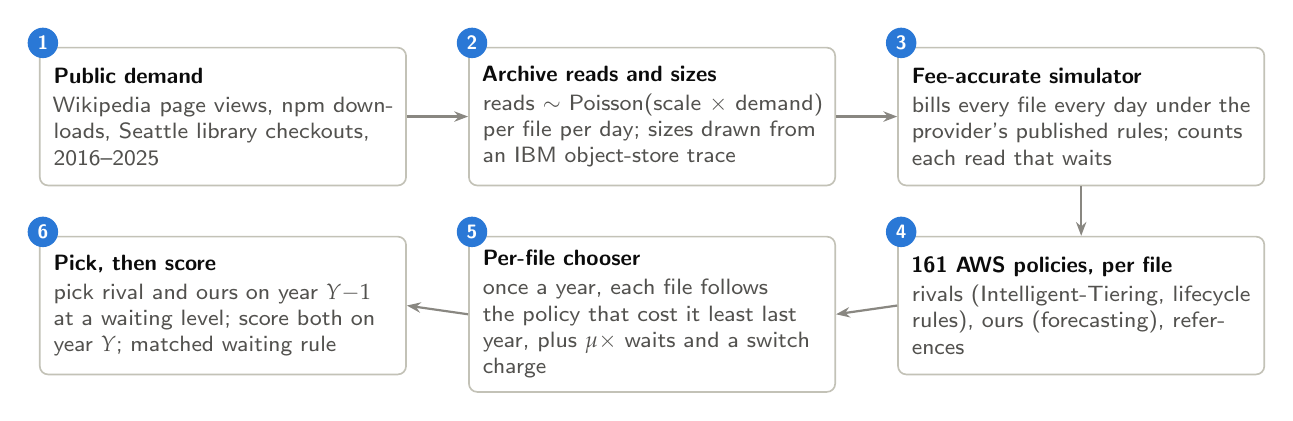
\begin{tikzpicture}[
  font=\sffamily\footnotesize,
  box/.style={draw=axisc, line width=0.6pt, rounded corners=3pt, fill=white, align=left,
              text width=4.3cm, minimum height=1.75cm, inner sep=5pt, anchor=north west},
  hd/.style={font=\sffamily\footnotesize\bfseries, text=inkc},
  arr/.style={-{Stealth[length=5pt]}, line width=0.8pt, color=mutedc},
  num/.style={circle, fill=oursc, text=white, font=\sffamily\scriptsize\bfseries, inner sep=1.2pt, minimum size=11pt}
]
\node[box] (a) at (0,0) {{\color{inkc}\textbf{Public demand}}\\[1pt]\color{ink2c}Wikipedia page views, npm downloads, Seattle library checkouts, 2016--2025};
\node[box] (b) at (5.45,0) {{\color{inkc}\textbf{Archive reads and sizes}}\\[1pt]\color{ink2c}reads $\sim$ Poisson(scale $\times$ demand) per file per day; sizes drawn from an IBM object-store trace};
\node[box] (c) at (10.9,0) {{\color{inkc}\textbf{Fee-accurate simulator}}\\[1pt]\color{ink2c}bills every file every day under the provider's published rules; counts each read that waits};
\node[box] (d) at (10.9,-2.4) {{\color{inkc}\textbf{161 AWS policies, per file}}\\[1pt]\color{ink2c}rivals (Intelligent-Tiering, lifecycle rules), ours (forecasting), references};
\node[box] (e) at (5.45,-2.4) {{\color{inkc}\textbf{Per-file chooser}}\\[1pt]\color{ink2c}once a year, each file follows the policy that cost it least last year, plus $\mu \times$ waits and a switch charge};
\node[box] (f) at (0,-2.4) {{\color{inkc}\textbf{Pick, then score}}\\[1pt]\color{ink2c}pick rival and ours on year $Y{-}1$ at a waiting level; score both on year $Y$; matched waiting rule};
\draw[arr] (a.east) -- (b.west);
\draw[arr] (b.east) -- (c.west);
\draw[arr] (c.south) -- (d.north);
\draw[arr] (d.west) -- (e.east);
\draw[arr] (e.west) -- (f.east);
\node[num] at ($(a.north west)+(0.05,0.05)$) {1};
\node[num] at ($(b.north west)+(0.05,0.05)$) {2};
\node[num] at ($(c.north west)+(0.05,0.05)$) {3};
\node[num] at ($(d.north west)+(0.05,0.05)$) {4};
\node[num] at ($(e.north west)+(0.05,0.05)$) {5};
\node[num] at ($(f.north west)+(0.05,0.05)$) {6};
\end{tikzpicture}

\caption{How every result is produced. Public demand becomes archive reads (1--2). The simulator bills each file under each of 161 policies (3--4). The per-file chooser combines them (5). The pick-then-score rule compares ours with the best rival on a year neither has seen (6).}
\label{fig:pipeline}
\end{figure}

\subsection{Datasets}

No public dataset records reads of an archive's files, so we use public demand series as stand-ins and map demand to reads (\cref{tab:data}). They differ in how predictable they are (\cref{fig:demand}). npm's within-year profile repeats: it rises steadily through each year and drops sharply at the end-of-year holidays. Wikipedia's is nearly flat, with spikes. The library's has no stable shape, and two events broke it: the 2020 closures, and a ransomware attack on the Seattle Public Library in late May 2024~\cite{spl_cyberattack}. In the sample, checkouts fell from about 4,000 a month in January to April 2024 to 1,114 in May and 670 in June.

\begin{table}[t]
\centering
\caption{Datasets. Counts are for the sealed years 2024 and 2025.}
\label{tab:data}
\small
\begin{tabularx}{\textwidth}{@{}l>{\raggedright\arraybackslash}Xrr@{}}
\toprule
Dataset & Source and sample & Files & Stored \\
\midrule
D1 Wikipedia & Daily user page views~\cite{wikimedia_pageviews} of 10,000 articles: the 5,000 most viewed and 5,000 at random & 9,684--9,867 & 0.19 TB \\
D3 npm & Daily downloads~\cite{npm_downloads} of 300 packages: the 100 most used and 200 at random from the next 4,900 & 295--298 & 4 GB \\
D4 Library & Monthly checkouts~\cite{seattle_checkouts} of a fixed random sample of 10,000 titles, spread evenly over each month & 10,000 & 0.21 TB \\
\bottomrule
\end{tabularx}
\end{table}

\begin{figure}[t]
\centering
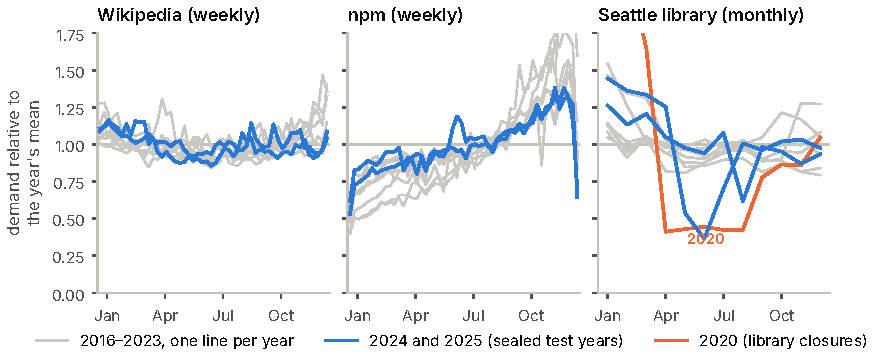
\includegraphics[width=\textwidth]{figures/fig3_demand.pdf}
\caption{Within-year demand of the average file, one line per year. Each file's demand is divided by its own mean for that year, then averaged over files. The sealed years (blue) look like earlier years on Wikipedia and npm. On the library data, 2020 (orange) and 2024 (the dip in May and June, during a ransomware attack on the library) break the pattern.}
\label{fig:demand}
\end{figure}

\paragraph{From demand to reads} Views and downloads are mostly served by caches and mirrors, not by an archive. We therefore draw each file's daily reads as $\text{Poisson}(s \cdot d)$, where $d$ is its demand that day and $s$ is one scale per dataset (one per cohort for Wikipedia). The central scale makes the median file read about 18 times a year, set on 2016--2022 data. The low and high settings use 10 times less and 10 times more. Draws come from fixed random streams, so every run is reproducible. A file exists from its first day of demand.

\paragraph{File sizes} None of the sources has file sizes. We draw them from the IBM object-store trace in the SNIA IOTTA repository~\cite{snia_ibm_trace} (central setting), with Wikimedia media sizes as the low setting and the trace's upper half as the high one. In the central setting the median file is 56--68~KB, the 99th percentile about 0.8~GB, and the largest about 1~GB.

Absolute bills are small, tens of dollars a year, because the samples are small. The comparisons are relative. Storage scales with bytes and request fees with files, so a larger archive with the same mix of sizes and reads would show the same percentages.

\subsection{Simulator}

The simulator takes, for each file, its size, its creation day and its reads per day, and a plan: which class the file is in each day, plus any restores ordered ahead of time. It returns a bill in ten categories: storage, archive overhead, temporary restored copies, early deletion, transitions, retrieval, restore requests, read requests, uploads and monitoring. It also returns every read that found its file frozen, with how long it waited. Rules are taken from the providers' documentation and quoted with their sources in the repository. They include minimum billable sizes, per-object archive overhead, restores and their temporary copies, and the managed services' own state machines.

\paragraph{Validation (gate G2)} Before any real data was used, the simulator matched 24 of 24 hand calculations to a relative error below $10^{-9}$ and 4 of 4 AWS Pricing Calculator readings to the cent. It caught 22 of 22 deliberately planted bugs. By the end of the project, the planted-bug check covered 48 bugs across the simulator, the policies and the protocol code, and caught all of them.

% =====================================================================================
\section{Methods compared}
\label{sec:methods}

All methods run on every file. Files never interact in the simulator, so a plan that gives each file its own policy costs exactly the sum of each file's cost under its policy. We simulate 161 AWS policies.

\paragraph{Rivals (19)} S3 Intelligent-Tiering in six settings (with and without its archive tiers); age-based lifecycle rules that move every file to one class 30 or 90 days after upload, for every class; and the archive rules again with bulk restores on demand. As on AWS, files under 128~KB never leave Standard under a lifecycle rule.

\paragraph{Ours (91, plus the chooser)} Every method of ours forecasts with last year's reads.
\begin{itemize}
  \item \emph{Seasonal-naive rule:} a file is warm if it was read in the same days last year (364 days back, same weekday) or recently. Otherwise it sits in a cold class, or stays archived with restored copies ordered ahead of the forecast reads, at standard or bulk speed.
  \item \emph{Fee-aware planner:} each day, puts each file in the class with the lowest expected cost over the next 30, 90 or 180 days, counting every fee.
  \item \emph{Intelligent-Tiering with forecast restores:} uses Intelligent-Tiering's archive tiers, and restores a file a set number of days before last year's reads say it will be wanted.
  \item \emph{Per-file chooser:} once a year, each file follows the policy (out of all 161, rivals included) with the lowest score
  \[
    \text{score}(p, i) = \text{cost}_{Y-1}(p, i) + \mu \cdot \text{waits}_{Y-1}(p, i) + \text{switch}(i)\cdot[p \neq p_{\text{now}}(i)],
  \]
  where cost and waits are file $i$'s bill and waited reads under policy $p$ last year. The switch charge is an upper bound on the one-off cost of moving the file (the dearest retrieval, request and early-deletion fees on the sheet). The file keeps its current policy unless the best score is lower by more than a margin $m$. Files without history stay on plain Intelligent-Tiering. There are 21 settings: $\mu \in \{0, 0.001, 0.01, 0.1, 1, 10\}$ USD per waited read, $m \in \{0, 0.1, 0.25\}$, and an ``online'' menu without policies under which reads can wait.
\end{itemize}

\paragraph{References (51, plus the ceiling)} Each of our rules has a \emph{reactive twin} with the forecast switched off, so a gain can be traced to the forecast rather than to reacting. The \emph{forecastable ceiling} makes the chooser's choice on an independent random draw of the scored year's reads from the same expected rates. It knows each file's true read rate, but not the draw that is scored. It shows how much a perfect forecast of rates could earn.

% =====================================================================================
\section{Protocol}
\label{sec:protocol}

\begin{figure}[t]
\centering
% Figure 2: which years each test used (TikZ, included by main.tex and by standalone.tex)
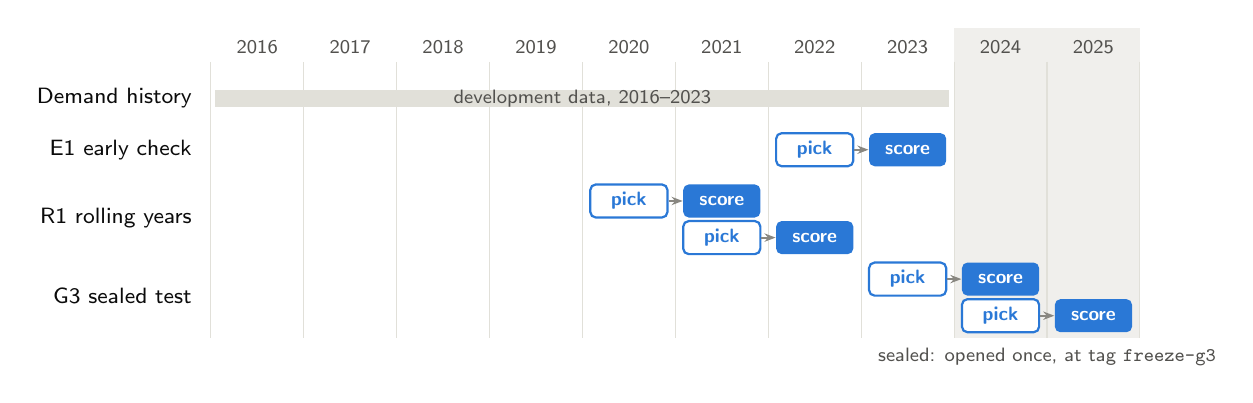
\begin{tikzpicture}[
  font=\sffamily\footnotesize, x=1.18cm, y=0.62cm,
  pick/.style={draw=oursc, line width=0.8pt, fill=white, rounded corners=2pt, minimum width=0.98cm, minimum height=0.42cm, inner sep=0pt, text=oursc, font=\sffamily\scriptsize\bfseries},
  score/.style={fill=oursc, rounded corners=2pt, minimum width=0.98cm, minimum height=0.42cm, inner sep=0pt, text=white, font=\sffamily\scriptsize\bfseries},
  arr/.style={-{Stealth[length=4pt]}, line width=0.7pt, color=mutedc},
  lab/.style={anchor=east, text=inkc, align=right, font=\sffamily\footnotesize}
]
% sealed band
\fill[washc] (8.5,-5.6) rectangle (10.5,0.75);
\node[text=ink2c, font=\sffamily\scriptsize, align=center] at (9.5,-6.0) {sealed: opened once, at tag \texttt{freeze-g3}};
% year axis
\foreach \y [count=\i] in {2016,...,2025} {
  \node[text=ink2c, font=\sffamily\scriptsize] at (\i,0.35) {\y};
  \draw[gridc, line width=0.4pt] (\i-0.5,0.05) -- (\i-0.5,-5.6);
}
\draw[gridc, line width=0.4pt] (10.5,0.05) -- (10.5,-5.6);
% rows
\node[lab] at (0.4,-0.7) {Demand history};
\fill[gridc] (0.55,-0.88) rectangle (8.45,-0.52);
\node[text=ink2c, font=\sffamily\scriptsize] at (4.5,-0.7) {development data, 2016--2023};
\node[lab] at (0.4,-1.75) {E1 early check};
\node[pick] (e1p) at (7,-1.75) {pick}; \node[score] (e1s) at (8,-1.75) {score};
\draw[arr] (e1p) -- (e1s);
\node[lab] at (0.4,-3.15) {R1 rolling years};
\node[pick] (r1a) at (5,-2.8) {pick}; \node[score] (r1b) at (6,-2.8) {score};
\draw[arr] (r1a) -- (r1b);
\node[pick] (r1c) at (6,-3.55) {pick}; \node[score] (r1d) at (7,-3.55) {score};
\draw[arr] (r1c) -- (r1d);
\node[lab] at (0.4,-4.75) {G3 sealed test};
\node[pick] (g1a) at (8,-4.4) {pick}; \node[score] (g1b) at (9,-4.4) {score};
\draw[arr] (g1a) -- (g1b);
\node[pick] (g2a) at (9,-5.15) {pick}; \node[score] (g2b) at (10,-5.15) {score};
\draw[arr] (g2a) -- (g2b);
% outcomes
\end{tikzpicture}

\caption{Which years each test used. Every method was picked on one year and scored on the next. The data loaders refused the sealed years 2024 and 2025; they were opened once, by code at the freeze tag.}
\label{fig:timeline}
\end{figure}

\paragraph{Pick, then score} A test is a set of \emph{lines}: a dataset, a waiting level, and a pair of years (pick on $Y{-}1$, score on $Y$). There are two waiting levels: L0, where no read may wait, and L1, where at most 1\% of reads may wait. On the pick year we choose the cheapest rival that meets the level. We then choose the cheapest of ours that waits no more than that rival. Both are scored on year $Y$. The \emph{gap} is $1 - \text{cost}_{\text{ours}} / \text{cost}_{\text{rival}}$. Under the deciding \emph{matched} rule, a line passes if the gap is at least 5\% and ours again waits on no more reads than the rival in year $Y$. A second rule, reported only, gives ours the full 1\% allowance.

\paragraph{Three tests (\cref{fig:timeline})} \emph{E1}, an early futility check, picked on 2022 and scored 2023 once. \emph{R1}, the gate for the per-file methods, used the rolling pairs 2020$\to$2021 and 2021$\to$2022. \emph{G3}, the sealed test, used 2023$\to$2024 and 2024$\to$2025. The order of work is visible in git: E1's picks were committed before 2023 was run (d1cf04d), R1's protocol before any real-data run (0bde4de), and G3's pre-registration in the commit the freeze tag points to (cc4b852).

\paragraph{The sealed years} The data loaders refused any file from 2024 or later by its folder name, and no analysis opened those years before the sealed test. For G3 the code opened them only when the tag \texttt{freeze-g3} existed on GitHub and locally, pointed at the running commit, and no tracked file had changed. The author created the tag on GitHub before the sealed files were copied in. Their hashes and modification times, all from 2026-10-29, are recorded with the results.

\paragraph{Pre-registered hypotheses} \Cref{tab:hyp} lists them. The proof of concept passes if (H1 or H2) and H5, H6, H7 and H9 all hold. The kill rule, also written in advance: if H1 and H2 both fail, the product thesis stops and the work becomes a paper.

\begin{table}[t]
\centering
\caption{Pre-registered hypotheses for the sealed test, and their outcome.}
\label{tab:hyp}
\small
\begin{tabularx}{\textwidth}{@{}l>{\raggedright\arraybackslash}X>{\raggedright\arraybackslash}p{4.6cm}@{}}
\toprule
& Passes if (sealed years, AWS, matched rule) & Result \\
\midrule
H1 Cost & At one level, both pairs: gap $\geq$ 5\%, ours waits no more than the rival, 95\% paired-bootstrap interval of the gap above zero (2,000 resamples over files). On at least 2 of the 3 datasets & \fail\ on all three \\
H2 Waiting & At L1, both pairs: ours costs no more, and its share of waited reads is at most half the rival's. On 2 of 3 & \fail\ on all three \\
H3 Headroom & Ours' gap divided by the ceiling's gap (reported) & 0.94 and 0.99 (Wikipedia); 0.76 and 1.99 (npm) \\
H4 Model needed & Ours against the seasonal-naive family alone (reported) & The seasonal-naive pick costs 0.6\% to 29\% more than the rival on all 12 lines \\
H5 Robust & The passing hypothesis holds in at least 8 of 10 scenarios & \fail: nothing passed in base. H1 held in 2 of 10, H2 in 1 \\
H6 Compute & Compute below 5\% of the saving (0.04 USD per core-hour) & 0.01\% to 0.13\%; not scored, since no dataset passed \\
H7 Simulator & Gate G2 & \pass \\
H9 Reproducible & A fresh clone at the tag reproduces every base line within 0.05\% & \pass: every line matched; run files byte-identical \\
\bottomrule
\end{tabularx}
\end{table}

\paragraph{Deviations} Three, all recorded before or as they happened. (1) Gate R1 failed (\cref{sec:r1}). By its rule the project should have stopped there. The author overrode it as a documented deviation: the methods were frozen unchanged and the sealed years opened once. R1 is reported as failed. (2) The library sample for 2024 and 2025 was extracted after the freeze, with the frozen extraction code. The same code first reproduced the pre-freeze 2023 sample exactly. (3) The workspace restarted during the ninth of ten scenarios. The run resumed from a checkout of the tag; the runs recomputed after the restart were byte-identical to those before it.

% =====================================================================================
\section{Results}
\label{sec:results}

\subsection{Early check (E1, 2023)}
E1 asked whether the simplest forecast showed any sign worth chasing. It passed by its own rule, but only against weak rivals. Every passing line was on Azure, against last-access rules on a locally redundant sheet where smart tier is not offered (Wikipedia +9.1\%, npm +23.1\%, library +26.1\%). Against Intelligent-Tiering and Autoclass, the seasonal-naive rule never passed: it lost by up to 69\%, or was within half a percent. A perfect forecast of the scored year beat Intelligent-Tiering by 4\% to 27\% at L0, but came within $-7\%$ to $+6\%$ of Autoclass. We therefore dropped Google and built the per-file methods for AWS.

\subsection{Rolling years (gate R1)}
\label{sec:r1}
R1 failed narrowly. The chooser was 27.6\% and 48.5\% cheaper than Intelligent-Tiering on Wikipedia, and 40.4\% and 43.4\% on npm, at L1. It passed both rolling lines on npm, but on Wikipedia in 2021 0.224\% of its reads waited against the rival's 0.218\%. On the library data it lost, after the 2020 closures broke the link between one year and the next (\cref{fig:results}, open markers).

\subsection{The sealed test (G3, 2024--2025)}

\begin{figure}[t]
\centering
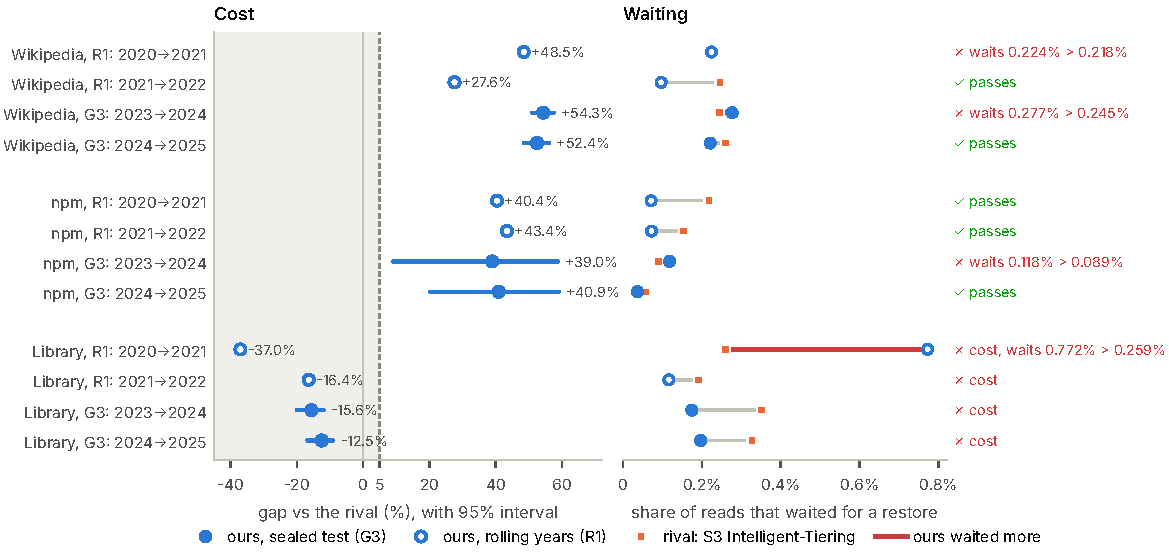
\includegraphics[width=\textwidth]{figures/fig4_results.pdf}
\caption{Every rolling (R1, open) and sealed (G3, filled) line at L1 under the matched rule. Left: how much cheaper ours was than the rival (S3 Intelligent-Tiering with its archive tiers), with the 95\% paired-bootstrap interval for the sealed years. Right: the share of reads that waited, ours against the rival. A line passes only if ours is at least 5\% cheaper and waits on no more reads. Wikipedia and npm failed in 2024 on waiting alone.}
\label{fig:results}
\end{figure}

\textbf{H1 and H2 failed on every dataset (\cref{tab:hyp}).} \Cref{fig:results} shows why. On Wikipedia and npm, the chooser was 52\% to 54\% and 39\% to 41\% cheaper than the rival, with 95\% intervals above zero. In 2024, though, slightly more of its reads waited than the rival's: 0.277\% against 0.245\% on Wikipedia, and 0.118\% against 0.089\% on npm. Each of those datasets failed one of its two sealed lines, and H1 needs both. On the library data, the cheapest of our policies that met the waiting rule on the pick year was Intelligent-Tiering with forecast restores. It lost by 15.6\% and 12.5\%. At L0, ours either equalled Intelligent-Tiering or, on npm in 2024, saved money only by letting a few reads wait. No L0 line passed.

\paragraph{Waiting in hours} The matched rule counts reads, not hours. Even on lines where ours waited on fewer reads, those reads waited longer: up to 48 hours (bulk restores from Deep Archive) against the rival's 12. In total, ours waited 2.9 to 4.3 times the rival's hours on the Wikipedia and npm lines. With the reported-only equal allowance, the gaps are similar (+54.3\% and +52.7\% on Wikipedia, +20.9\% and +49.3\% on npm), but ours then waits on up to five times the rival's share of reads, and for up to 7.9 times its hours (\cref{tab:equal} in the appendix).

\paragraph{Seasonality alone (H4)} Picked by the same rule, the seasonal-naive family cost 0.6\% to 29\% more than the rival on all twelve base lines. Applied to every file, the forecast loses. The per-file chooser does use seasonal policies, but only for a minority of files (\cref{sec:why}).

\paragraph{Azure} On Azure's zone-redundant sheet, where smart tier is offered and there is no archive tier, no read ever waits. There the chooser only ties smart tier: it is 0.02\% to 0.10\% cheaper in the sealed years.

\paragraph{Reproduction (H9)} A fresh clone of the tag re-simulated and re-scored the base scenario. Every rival and ours cost matched, and the run files compared were byte-identical.

% =====================================================================================
\section{Why it fails}
\label{sec:why}

\subsection{Where the money is}

\begin{figure}[t]
\centering
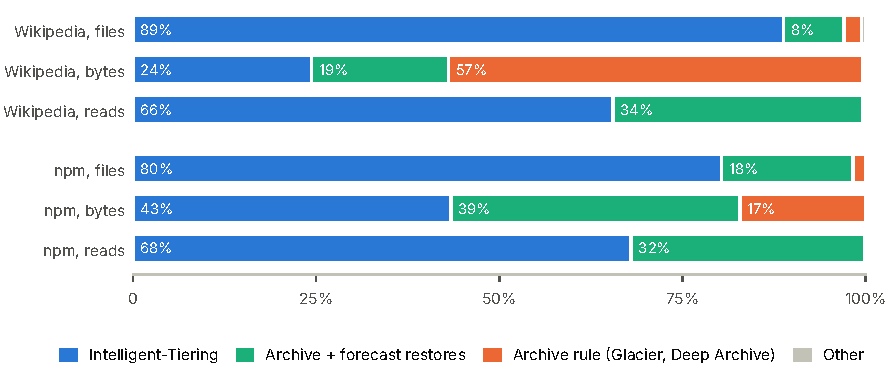
\includegraphics[width=\textwidth]{figures/fig6_allocation.pdf}
\caption{What the chooser did with the files in its 2024 sealed picks: the share of files, bytes and reads under each kind of policy. On Wikipedia, 2.4\% of the files (median 318 MB) went to plain archive rules. They hold 57\% of the bytes and receive 0.25\% of the reads.}
\label{fig:allocation}
\end{figure}

\Cref{fig:allocation} shows how the chooser made its saving. It left 80\% to 89\% of files on Intelligent-Tiering. It moved 8\% to 18\% of files, mid-sized ones that are read regularly, to archive with forecast restores. It sent a few very large, rarely read files to plain Glacier or Deep Archive rules; on Wikipedia, most of them with bulk restores. On Wikipedia in 2024 that last group was 232 of 9,684 files, with a median size of 318~MB. It held 57\% of the bytes and received 0.25\% of the reads. Storage is billed by the byte, so these few files decide most of the storage bill.

So the saving is mostly per-file economics rather than seasonality. Most of the bytes go to plain archive rules that need no forecast at all; the forecasting policies help only for the minority of files they are given. A file that is large, rarely read and read by someone willing to wait is far cheaper in Deep Archive than in any tier Intelligent-Tiering will put it in by itself. The chooser finds these files from last year's bill. What it cannot do is promise that next year's readers of those files will be as few as last year's.

\subsection{The waiting line, and the ceiling}

\begin{figure}[t]
\centering
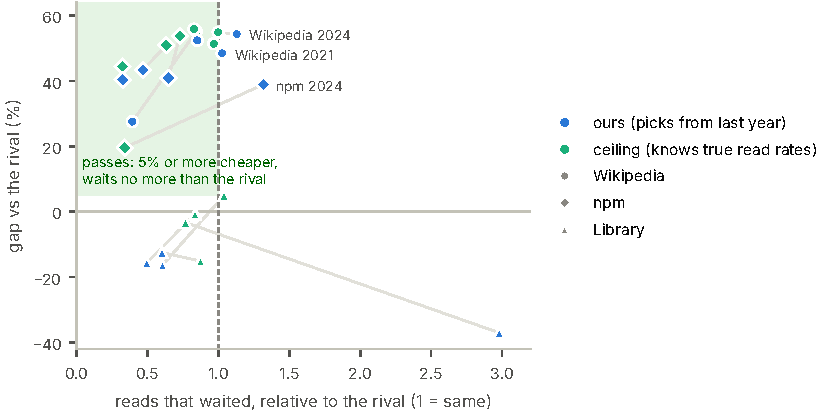
\includegraphics[width=0.86\textwidth]{figures/fig5_pass_region.pdf}
\caption{Each L1 line of R1 and G3, for ours (blue) and the forecastable ceiling (green), joined by a grey line. Horizontal axis: reads that waited, relative to the rival. Vertical axis: the gap. The ceiling, which knows each file's true read rate, lands in the passing region on all eight Wikipedia and npm lines. Ours crosses the waiting line three times.}
\label{fig:pass}
\end{figure}

The chooser picks the setting whose waits on the pick year were no more than the rival's, and hopes the next year behaves the same. In one of the two sealed years it did not, on both datasets, and the same had happened once in R1. The forecastable ceiling makes the same kind of choice, but from each file's true expected read rate instead of last year's draw. It waited no more than the rival on all eight Wikipedia and npm lines of R1 and G3, while 20\% to 56\% cheaper (\cref{fig:pass}). A good enough forecast of each file's \emph{rate} would therefore have passed. Last year's reads were not one.

On the library data, even the ceiling's gap ranged from +4.9\% to $-15.1\%$. Knowing the rates does not help when the rates themselves shift. This happened twice: with the 2020 closures, and with the 2024 cyberattack, which fell inside the sealed test.

\subsection{Robustness}

\begin{figure}[t]
\centering
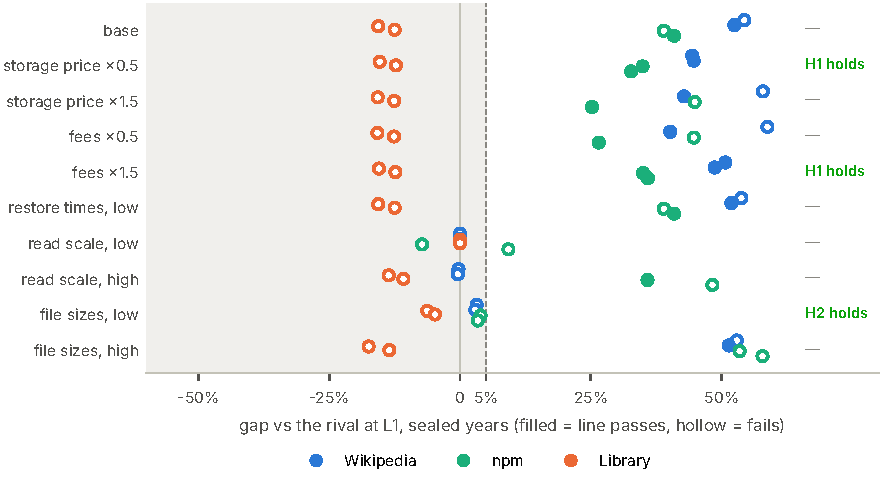
\includegraphics[width=\textwidth]{figures/fig7_scenarios.pdf}
\caption{The four Wikipedia and npm sealed lines and two library lines at L1, in each of the ten pre-registered scenarios. Filled markers pass; hollow ones fail. The gap is large in most scenarios. Whether a line passes changes from scenario to scenario. H1 held in two scenarios and H2 in one; H5 needed eight.}
\label{fig:scen}
\end{figure}

\Cref{fig:scen} repeats the sealed test in the ten pre-registered scenarios. These were storage prices and fees at 0.5 and 1.5 times, restore times at the low end of AWS's range, read scale and file sizes low and high. The pattern is the same throughout: large gaps on Wikipedia and npm, losses on the library, and passes that come and go. With storage at half price or fees at 1.5 times, the chosen settings waited no more than the rival in both sealed years, and H1 held. With small files the gaps shrank to about 3\%, but ours almost never made a reader wait (at most 0.007\% of reads, against 0.03\% to 0.11\% for the rival), so H2 held. Even if base had passed, H5 (8 of 10) would have failed.

% =====================================================================================
\section{Discussion}
\label{sec:discussion}

\paragraph{For practitioners} Two results are useful whatever one thinks of forecasting. First, S3 Intelligent-Tiering is a strong default: no rule of ours applied to all files beat it, and with no waiting allowed nothing did. Second, a large share of a bill can sit in a small number of large, rarely read files. For those files, a plain Deep Archive rule with bulk restores is far cheaper, if their readers can wait up to two days. Finding them needs only last year's per-file bill, which a fee-accurate simulation provides.

\paragraph{What would change the answer} (1) A controller that holds waiting under a budget \emph{during} the year, rather than only at the yearly choice. This was planned as the next stage and not built after R1 failed. The ceiling suggests the target is reachable on stable data. The sealed years are spent, so testing it needs a new pre-registered test on later data. (2) A real archive's access log. Our reads are public demand scaled to archive levels; a real archive with large, seldom-read files would favour the per-file choice, and one with small or busy files would not. (3) A different notion of waiting. If waiting is judged in hours, ours looks worse. If a two-day restore is acceptable for the files in question, the saving stands without the waiting rule.

\paragraph{On pre-registration} The test failed by 0.03 percentage points of waited reads, on lines that were 39\% to 54\% cheaper. It is tempting to call that a pass in spirit. We do not, for two reasons. The same overshoot happened in R1, so it is a property of the method rather than bad luck. And a rule that can be relaxed after the data is seen gives no protection at all. The failure is what makes the rest of the evidence credible.

% =====================================================================================
\section{Threats to validity}
\label{sec:threats}

\begin{itemize}
  \item \textbf{No customer log.} Reads are mapped from public demand by a stated scale, and sizes are drawn from one trace. A real archive could favour either side.
  \item \textbf{Small sample.} Three datasets, two rolling and two sealed pairs. npm has fewer than 300 files, so its intervals are wide (lower ends +9.1\% and +20.3\%).
  \item \textbf{The waiting rule counts reads, not hours} (\cref{sec:results}).
  \item \textbf{A deviation was taken.} The sealed test ran only because the author overrode a failed gate. It was pre-registered and frozen first, but it is not the path the stop rule prescribed.
  \item \textbf{The switch charge is an upper bound,} conservative for ours.
  \item \textbf{One region per cloud, list prices.} Discounts, other regions and later price changes are not modelled; the price scenarios cover part of this.
  \item \textbf{AWS only for the per-file methods.} Google was dropped after E1. Azure was tested only against smart tier on a sheet without an archive tier.
  \item \textbf{Single author.} The hand calculations have not yet been re-derived by a second person. H9 was reproduced in the same kind of workspace, not on an independent machine.
\end{itemize}

% =====================================================================================
\section{Conclusion}

Forecasting seasonal demand did not beat reactive cloud auto-tiering in a test whose rules were fixed before the data was seen. Managed tiering beat every forecasting rule we applied to all files, because it moves data between its own tiers without the fees a do-it-yourself plan pays. The saving that remains is real and large, 39\% to 54\% on two of three datasets. It comes mainly from leaving a few large, rarely read files in deep archive, and its price is that their readers wait up to two days. A year-ahead choice cannot keep that waiting at the rival's level every year, and a sudden change in demand removes the saving altogether. The open question is whether a controller that budgets waiting within the year could keep the saving without the risk. That needs new data and a new pre-registered test.

% =====================================================================================
\section*{Artifact availability}
\addcontentsline{toc}{section}{Artifact availability}

Code, protocols, the decision log, per-run outputs and this paper's figures are at \url{https://github.com/summitkhatiwada22/seasonal-tiering-poc}~\cite{repo}. Code is released under the MIT licence, and the paper and documentation under CC BY 4.0. The sealed test runs from the tag \texttt{freeze-g3}:
\begin{center}
\small\ttfamily
\begin{tabular}{l}
git checkout freeze-g3 \\
uv run python -m sat.experiments.g3 run --workers 2 \\
uv run python -m sat.experiments.g3 score \\
uv run python -m sat.experiments.g3 reproduce --workers 2 \\
\end{tabular}
\end{center}
The raw data are public and are not redistributed; each downloaded file is recorded with its SHA-256 in the repository. \texttt{docs/RESULTS.md} lists every number in this paper with its source file. Figures are drawn by \texttt{scripts/paper/figures.py}.

\section*{Use of AI}
\addcontentsline{toc}{section}{Use of AI}

The research question is the author's. So are the decision to pre-register, every gate decision (including the override of R1), and the interpretation. The code, analyses, figures and drafts of this text were produced with the help of Claude (Anthropic), an AI model, working under the author's direction. Every decision is logged in the repository's \texttt{docs/DECISIONS.md}, and the full history of the work is in its git log. The author takes responsibility for the content.

\bibliographystyle{abbrvnat}
\setlength{\bibsep}{2pt}
{\small\bibliography{refs}}

% =====================================================================================
\appendix
\section{Additional results}

\begin{table}[H]
\centering
\caption{Sealed lines under the reported-only equal allowance (ours may use the full 1\%).}
\label{tab:equal}
\footnotesize
\begin{tabular}{@{}llrrrr@{}}
\toprule
Dataset & Years & Gap & Reads waited (rival / ours) & Wait hours (rival / ours) & Longest wait \\
\midrule
Wikipedia & 2023, 2024 & +54.3\% & 0.245\% / 0.277\% & 19,740 / 72,554 & 12 / 48 h \\
Wikipedia & 2024, 2025 & +52.7\% & 0.260\% / 0.242\% & 20,731 / 64,373 & 12 / 48 h \\
npm & 2023, 2024 & +20.9\% & 0.089\% / 0.447\% & 381 / 2,916 & 12 / 48 h \\
npm & 2024, 2025 & +49.3\% & 0.056\% / 0.082\% & 269 / 2,112 & 12 / 48 h \\
Library & 2023, 2024 & $-0.6$\% & 0.351\% / 0.629\% & 11,063 / 32,316 & 12 / 48 h \\
Library & 2024, 2025 & $-5.3$\% & 0.327\% / 0.923\% & 10,236 / 47,592 & 12 / 48 h \\
\bottomrule
\end{tabular}
\end{table}

\begin{table}[H]
\centering
\caption{Sealed lines at L1 under the matched rule: costs (USD per year for the sample) and waiting.}
\label{tab:sealed}
\footnotesize
\setlength{\tabcolsep}{4pt}
\begin{tabular}{@{}llrrrrr@{}}
\toprule
Dataset & Years & Rival & Ours & Gap (95\% interval) & Waited (rival / ours) & Hours (rival / ours) \\
\midrule
Wikipedia & 2023, 2024 & 35.874 & 16.380 & +54.3\% (51.0, 57.5) & 0.245\% / 0.277\% & 19,740 / 72,554 \\
Wikipedia & 2024, 2025 & 35.793 & 17.028 & +52.4\% (48.6, 56.0) & 0.260\% / 0.221\% & 20,731 / 59,755 \\
npm & 2023, 2024 & 0.624 & 0.381 & +39.0\% (9.1, 58.8) & 0.089\% / 0.118\% & 381 / 1,632 \\
npm & 2024, 2025 & 0.744 & 0.440 & +40.9\% (20.3, 59.0) & 0.056\% / 0.036\% & 269 / 972 \\
Library & 2023, 2024 & 12.530 & 14.490 & $-15.6$\% ($-19.9$, $-12.0$) & 0.351\% / 0.174\% & 11,063 / 5,026 \\
Library & 2024, 2025 & 11.962 & 13.456 & $-12.5$\% ($-16.8$, $-9.0$) & 0.327\% / 0.197\% & 10,236 / 5,850 \\
\bottomrule
\end{tabular}
\end{table}

\end{document}
